% Created 2018-05-03 Thu 08:37
% Intended LaTeX compiler: pdflatex
\documentclass[10pt]{beamer}
\usepackage[utf8]{inputenc}
\usepackage[T1]{fontenc}
\usepackage{graphicx}
\usepackage{grffile}
\usepackage{longtable}
\usepackage{wrapfig}
\usepackage{rotating}
\usepackage[normalem]{ulem}
\usepackage{amsmath}
\usepackage{textcomp}
\usepackage{amssymb}
\usepackage{capt-of}
\usepackage{hyperref}
\usetheme{Boadilla}
\author{ECON 499: Growth and Development}
\date{Spring 2018}
\title{Productivity}
\usecolortheme{seagull}
\usefonttheme[onlylarge]{structurebold}
\usefonttheme[onlymath]{serif}
\setbeamerfont*{frametitle}{size=\normalsize,series=\bfseries}
\setbeamertemplate{navigation symbols}{}
\setbeamertemplate{itemize item}[triangle]
\setbeamertemplate{footline}{}
\setbeamertemplate{enumerate items}[default]
\hypersetup{
 pdfauthor={ECON 499: Growth and Development},
 pdftitle={Productivity},
 pdfkeywords={},
 pdfsubject={},
 pdfcreator={Emacs 25.2.2 (Org mode 9.1.6)}, 
 pdflang={English}}
\begin{document}

\maketitle

\begin{frame}[label={sec:org2cda533}]{}
\alert{Announcements}
\begin{itemize}
\item Reading
\begin{itemize}
\item Chapter 7
\end{itemize}
\item Homework due Friday
\item Midterm next Thursday
\end{itemize}
\end{frame}

\begin{frame}[label={sec:org04ea2af}]{}
\alert{Explaining cross-country differences}
\begin{itemize}
\item So far: \(Y_t = K_t^\alpha (h_tL_t)^{1-\alpha}\)
\item We've tried to explain cross-country differences in terms of population growth, physical capital, human capital
\item Large differences remain
\item Factor accumulation alone not enough to explain differences in growth an income
\end{itemize}
\end{frame}

\begin{frame}[label={sec:org74d3219}]{Physical Capital Predicted vs Actual}
\begin{center}
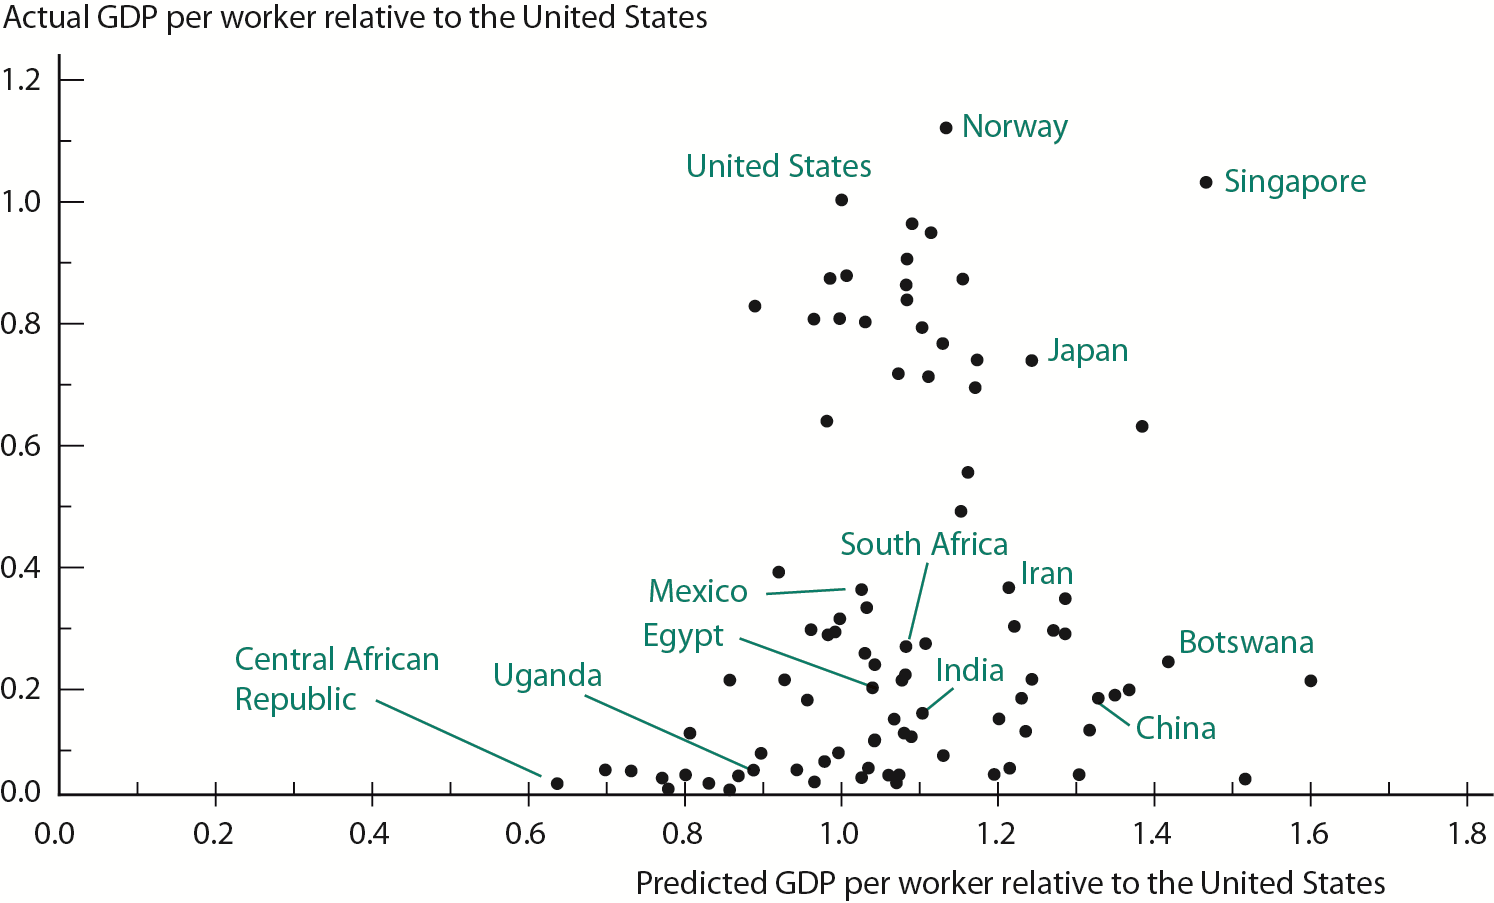
\includegraphics[width=.75\textwidth]{./img/3.7.png}
\end{center}
\end{frame}

\begin{frame}[label={sec:org19f2a0b}]{Human Capital Predicted vs Actual}
\begin{center}
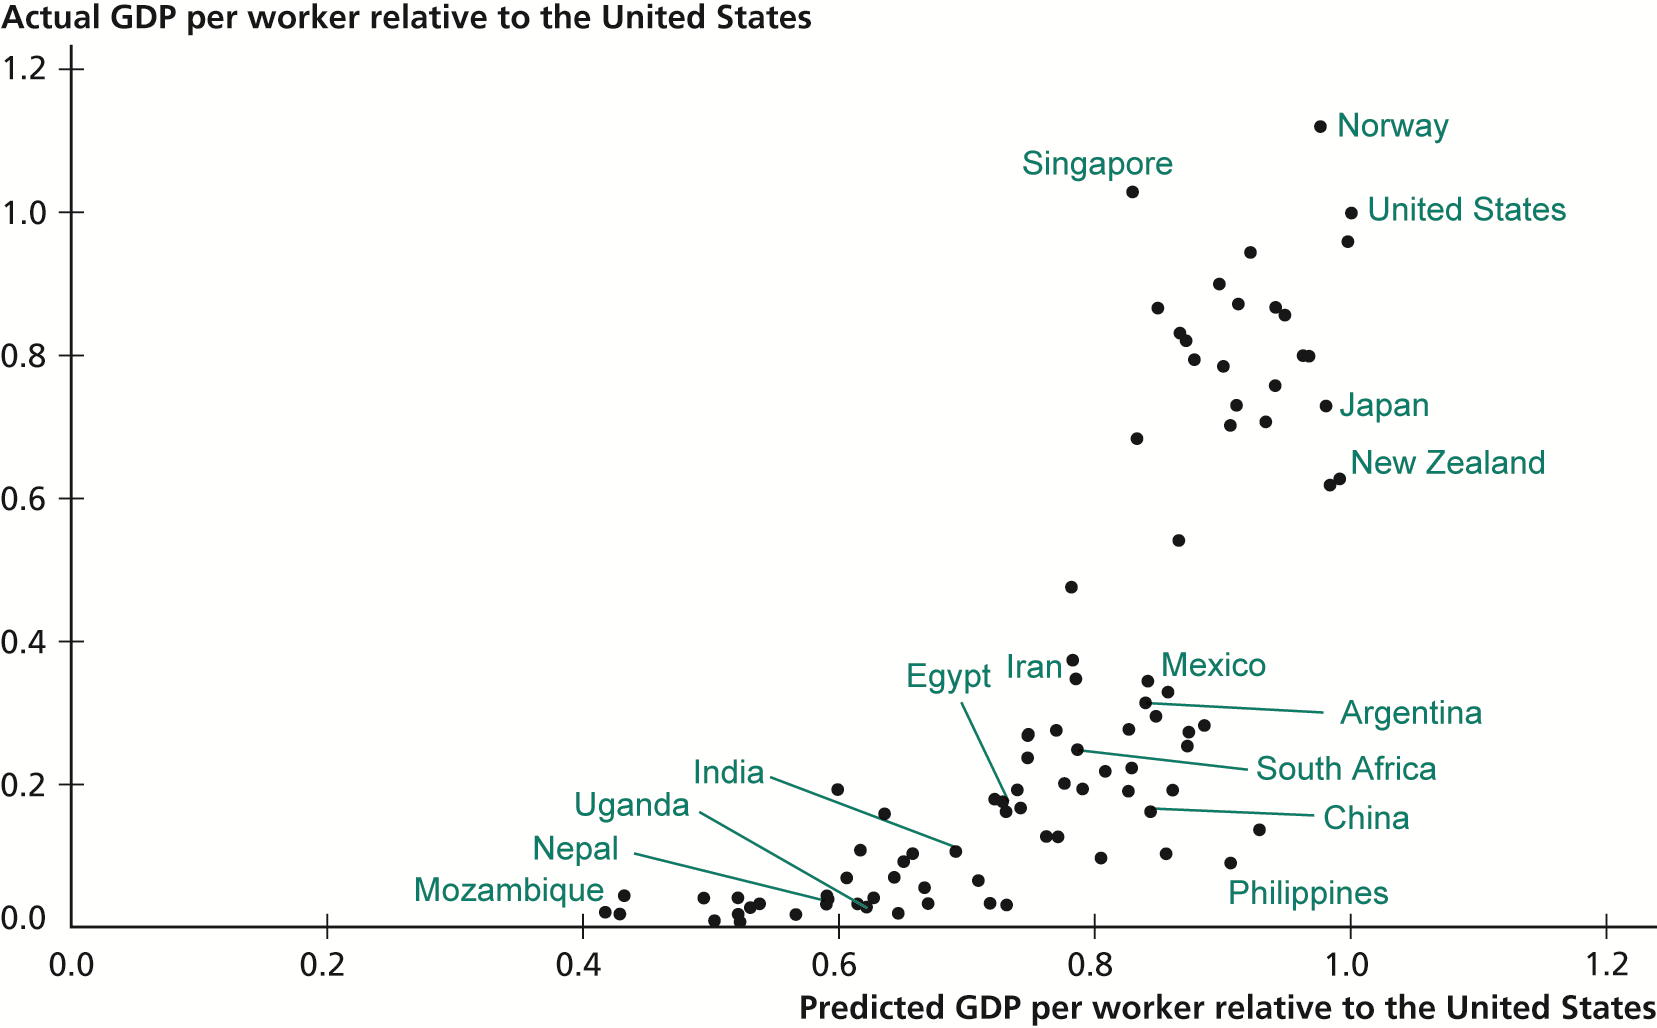
\includegraphics[width=.75\textwidth]{./img/6.12.png}
\end{center}
\end{frame}

\begin{frame}[label={sec:orgea028f4}]{}
\alert{Productivity}
\begin{itemize}
\item Some countries might be better at combining factors into output
\item Technology, efficiency, work-ethic, etc
\item How effective a country is at turning factors into output is called \alert{productivity}
\item Problem: Productivity is not directly observed, we must infer from other data using "accounting" techniques
\end{itemize}
\end{frame}

\begin{frame}[label={sec:org80a98ec}]{}
\begin{center}

\includegraphics[width=.75\textwidth]{./img/tab7.2.png}
\end{center}
\end{frame}

\begin{frame}[label={sec:org931c509}]{}
\begin{center}
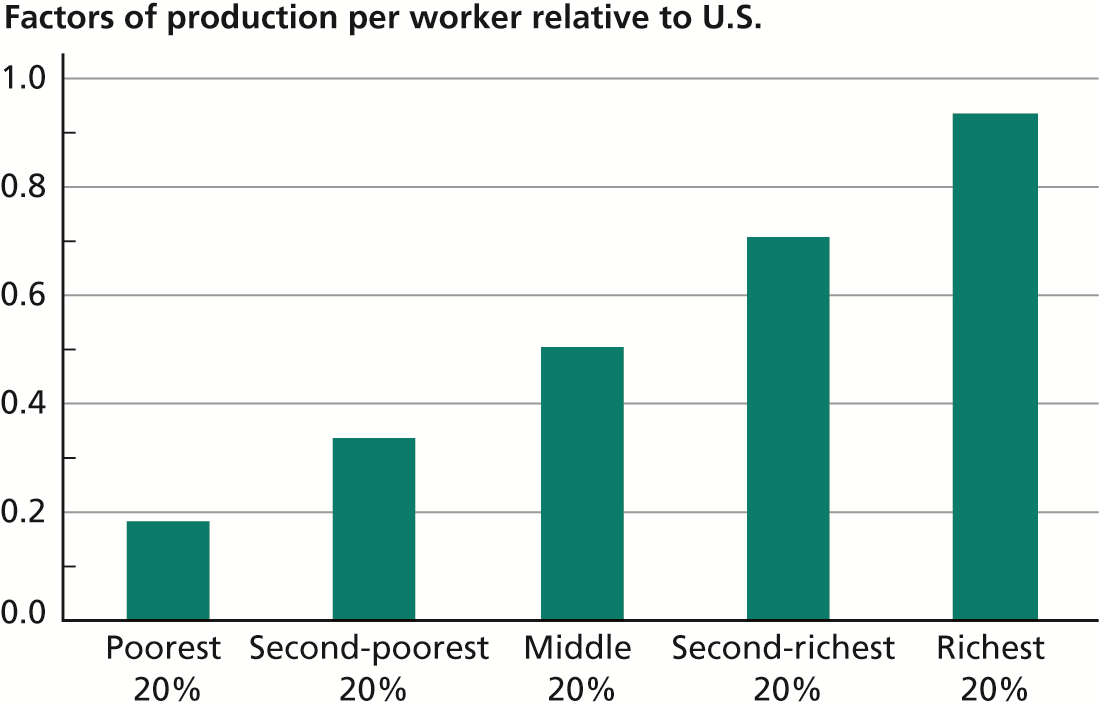
\includegraphics[width=.75\textwidth]{./img/7.3.png}
\end{center}
\end{frame}

\begin{frame}[label={sec:orgbf720d6}]{}
\begin{center}
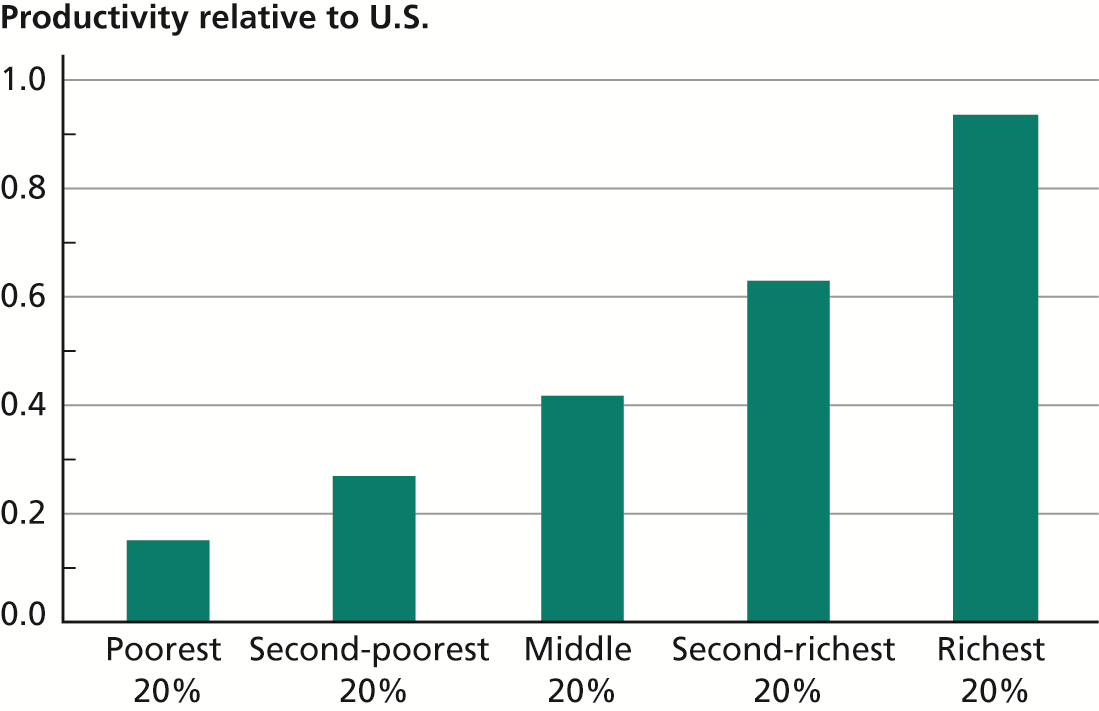
\includegraphics[width=.75\textwidth]{./img/7.4.png}
\end{center}
\end{frame}

\begin{frame}[label={sec:org9d1dc9d}]{}
\alert{Productivity and income}
\begin{itemize}
\item A large amount of the difference in income across countries is explained by productivity differences
\item Rich countries are more productive than poor countries
\item Productivity and factor accumulation are (roughly) equally responsible for cross-country income differences
\end{itemize}
\end{frame}

\begin{frame}[label={sec:orgee37c83}]{}
\begin{center}
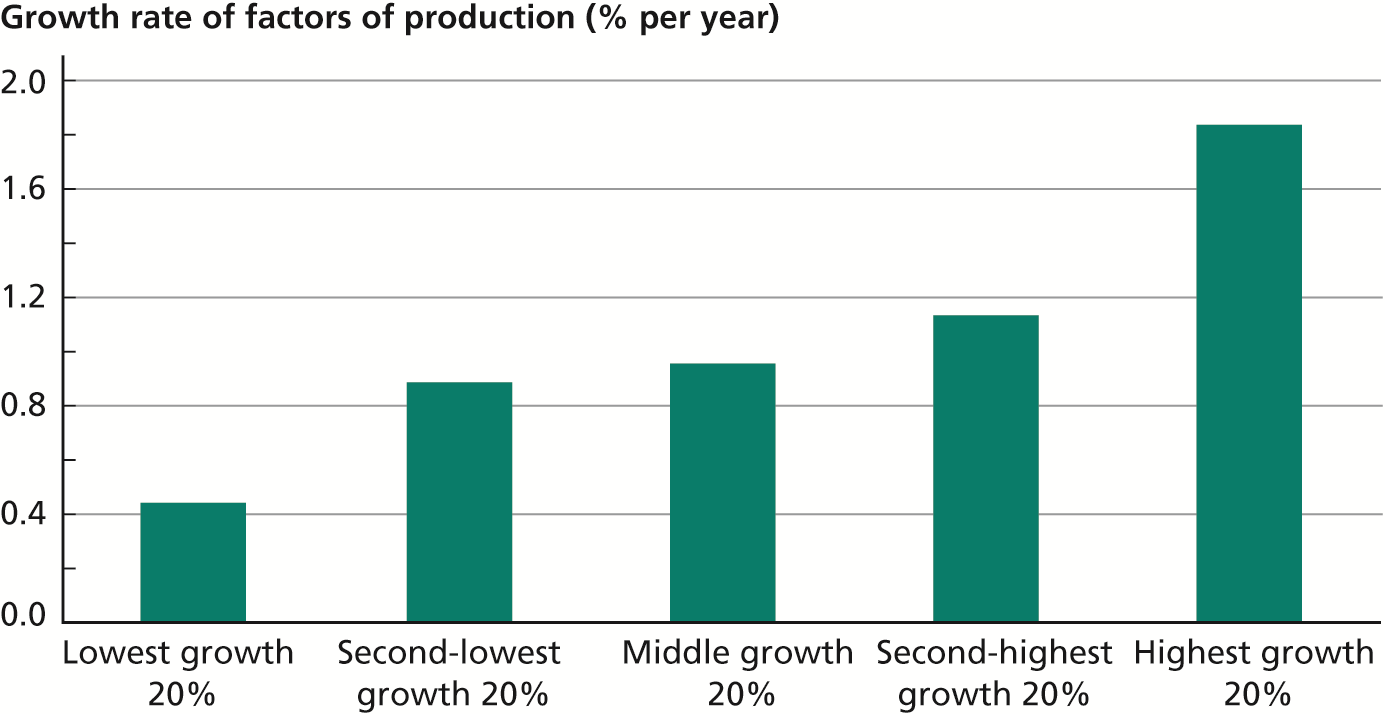
\includegraphics[width=.75\textwidth]{./img/7.5.png}
\end{center}
\end{frame}

\begin{frame}[label={sec:org81b6af0}]{}
\begin{center}
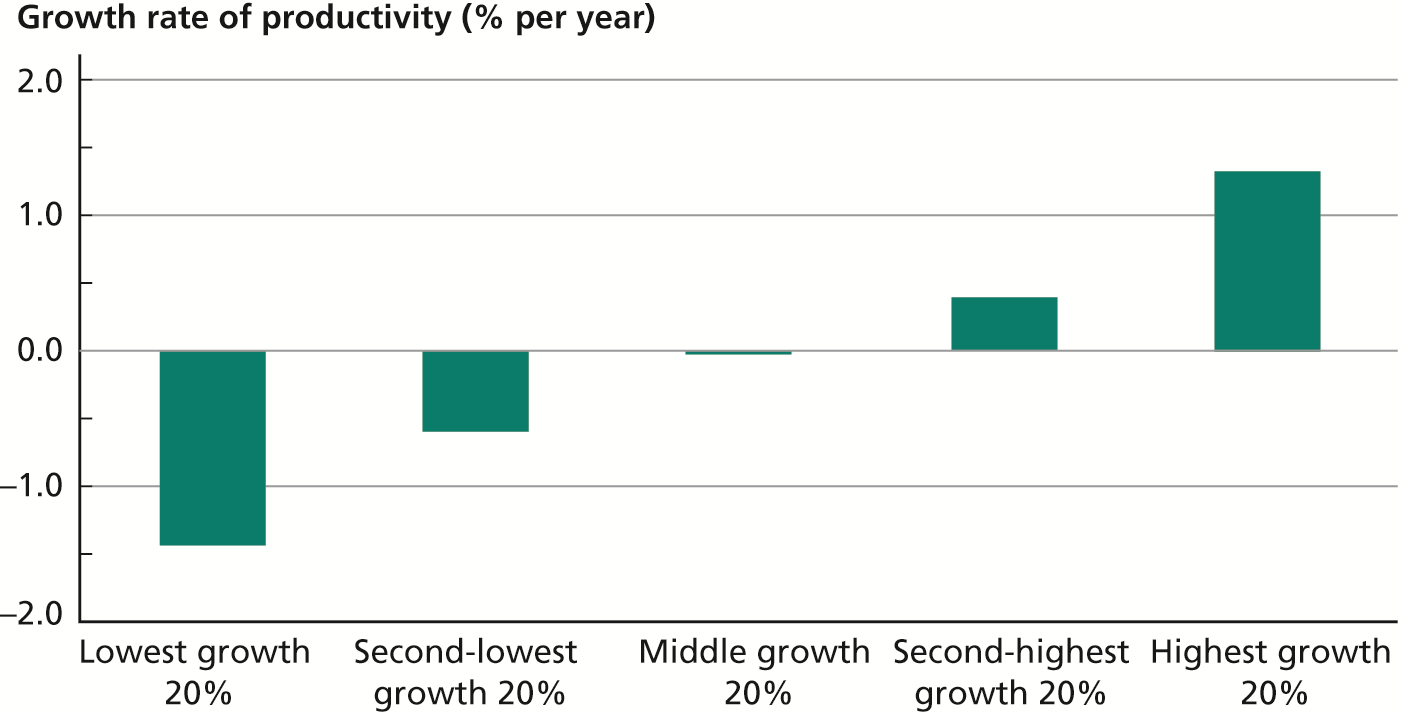
\includegraphics[width=.75\textwidth]{./img/7.6.png}
\end{center}
\end{frame}

\begin{frame}[label={sec:org1b7c909}]{}
\alert{Productivity and growth}
\begin{itemize}
\item Factor growth and productivity growth contribute to income per capita growth
\item Productivity growth relatively more important at explaining differences in income growth
\item Countries with lowest growth have negative productivity growth, despite positive factor growth
\item Low-growth countries are getting \alert{worse} at transforming factors into output over time
\end{itemize}
\end{frame}
\end{document}